\chapter{NumPy e Matplotlib}\label{numpy}

A lista (\inlcode{list}) em Python é uma estrutura de dados altamente versátil: cada elemento pode conter qualquer tipo
de objeto, independentemente do tamanho ou tipo, e a estrutura pode ser modificada e redimensionada dinamicamente.
No entanto, toda essa generalidade e flexibilidade tem um custo, especialmente em termos de desempenho.

Diferente de outras linguagens, o Python não possui um tipo embutido para representar \inlcode{arrays} no sentido
tradicional, ou seja, coleções de dados homogêneos com tamanho fixo.
Esse tipo de estrutura, embora bem mais restrita que uma lista, permite otimizações tanto no uso de memória quanto
na performance.

Isso torna-se particularmente crítico quando lidamos com grandes volumes de dados numéricos em aplicações
científicas, como regressão, otimização, álgebra linear os demais métodos utilizados em
computação científica.
Nessas situações, a eficiência no processamento é essencial, exigindo estruturas de dados mais especializadas e
performáticas que as listas tradicionais do Python.

A solução mais amplamente adotada para esse desafio em Python é o uso da biblioteca \inlcode{NumPy}, que, embora não
venha incluída por padrão na instalação da linguagem, consolidou-se como o padrão de fato no meio científico para
computação numérica.
Complementarmente, a biblioteca \inlcode{Matplotlib} é amplamente utilizada para visualização de dados através da
geração de gráficos (\inlcode{plots}).


Como \inlcode{NumPy} e \inlcode{Matplotlib} não fazem parte da biblioteca padrão, é necessário instalá-los manualmente.
Isso pode ser feito utilizando o \inlcode{pip}, o gerenciador de pacotes oficial do Python.
Para realizar a instalação, basta executar o seguinte comando no terminal:
\begin{minted}[escapeinside=??]{text}
?\textcolor{green!20!brown}{C:\char92curso\_python\char92>}? pip install numpy matplotlib
\end{minted}

Além disso, a biblioteca \inlcode{NumPy} fornece a estrutura de dados \inlcode{ndarray}, que permite representar
\inlcode{arrays} multidimensionais de forma compacta e eficiente.
Ela também disponibiliza um vasto conjunto de funções vetorizadas otimizadas, capazes de aplicar operações matemáticas
diretamente sobre todo o \inlcode{array}, dispensando o uso de laços explícitos que podem ser pouco performáticos em Python.
Essa abordagem vetorizada resulta em cálculos muito mais rápidos, especialmente ao lidar com grandes volumes de dados.


Veja o exemplo:
\begin{minted}[linenos]{custompython}
import numpy as np

x = np.linspace(0, 3, 7)
y = x**2 - 2*x

print(f"{x = }")
print(f"{y = }")
\end{minted}
\begin{minted}{text}
x = array([0. , 0.5, 1. , 1.5, 2. , 2.5, 3. ])
y = array([ 0.  , -0.75, -1.  , -0.75,  0.  ,  1.25,  3.  ])
\end{minted}

Na \textbf{linha 1}, declaramos que utilizaremos o pacote \inlcode{numpy}, e o faremos por meio do \emph{alias}
\inlcode{np}.
Ou seja, para não repetirmos \inlcode{numpy} diversas vezes ao longo do código, atribuímos a ele o nome
abreviado \inlcode{np}.

Na \textbf{linha 3}, utilizamos o método \inlcode{linspace} da biblioteca \inlcode{numpy} para criar um \inlcode{array}
contendo \inlcode{7} valores do tipo \inlcode{float}, igualmente espaçados no intervalo fechado de \inlcode{0} a
\inlcode{3} --- ou seja, incluindo os dois extremos do intervalo.


Na \textbf{linha 4}, exploramos as funcionalidades de vetorização da biblioteca \inlcode{NumPy} para aplicar a
expressão matemática diretamente a todos os elementos do \inlcode{array x}.
O resultado é um novo \inlcode{array y}, de mesmo tamanho, cujos valores correspondem à aplicação da expressão
$y_n = x_n^2 - 2x_n$ em cada elemento $x_n$ do \inlcode{array x}, sem a necessidade de laços explícitos.

Com uma pequena modificação no código, também podemos utilizar o pacote \inlcode{matplotlib} para gerar um gráfico que
representa os vetores \inlcode{x} e \inlcode{y} no plano cartesiano.
\begin{minted}{custompython}
import numpy as np
import matplotlib.pyplot as plt

# gera valores para os eixos x e y do gráfico
x = np.linspace(0, 3, 100)
y = x**2 - 2*x

# plota o gráfico
plt.plot(x,y)
plt.show()
\end{minted}

Esse código gera e exibe a figura:
\begin{center}
    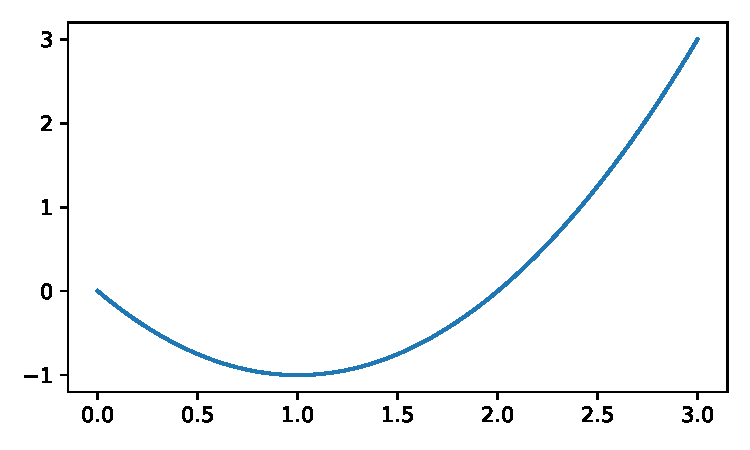
\includegraphics[scale=1.0]{figs/parabola}
\end{center}

A figura gerada exibe o gráfico construído a partir dos pares ordenados $(x_n, y_n)$.
Embora seja uma visualização simples, a biblioteca \inlcode{matplotlib} oferece uma ampla variedade
de funções auxiliares para personalizar o aspecto visual do gráfico.

O exemplo a seguir demostra algumas dessas funcionalidades:
\begin{minted}[linenos]{custompython}
import numpy as np
import matplotlib.pyplot as plt

# gera pontos para os eixo x e y
theta = np.linspace(0, 3*np.pi, 100)
y1 = np.sin(theta)
y2 = 0.7 * np.sin(theta - np.pi/3)
y3 = y1 + y2

# descomete caso queira fidelidade de fontes com Latex (necessário instalar Latex)
#plt.rcParams.update({'text.usetex': True, 'font.family': 'serif'})

plt.figure(figsize=(5, 2.8))    # define o latgura e altura da figura em polegadas
plt.plot(theta, y1, color='olivedrab' , linestyle='-.', label=r'$y_1$')     # plota y1
plt.plot(theta, y2, color='steelblue' , linestyle='--', label=r'$y_2$')     # plota y2
plt.plot(theta, y3, color='darkorange', linewidth=1.8 , label=r'$y_1+y_2$') # plota y3
plt.title('Gráfico de Exemplo')       # adiciona título ao gráfico
plt.xlabel(r'$\theta$ (radianos)')    # adiciona identificação do eixo x
plt.ylabel(r'$y(\theta)$')            # adiciona identificação do eixo y
plt.xlim(theta[0], theta[-1])         # define os limites do eixo x
plt.ylim(1.2*y3.min(), 1.2*y3.max())  # define os limites do eixo y
plt.grid(True)       # exibe grade
plt.legend()         # exibe legenda (valores atribuidos a plabel no plot)
plt.tight_layout()   # ajusta o grafico gerado aos limites da figura

# define os ticks do eixo x manualmente como múltiplos de π
xticks = [0, np.pi/2, np.pi, 3*np.pi/2, 2*np.pi, 5*np.pi/2, 3*np.pi]
xtick_labels = [r'0', r'$\frac{\pi}{2}$', r'$\pi$', r'$\frac{3\pi}{2}$',
                r'$2\pi$', r'$\frac{5\pi}{2}$', r'$3\pi$']
plt.xticks(xticks, xtick_labels)

# exporta a figura gerada para um arquivo externo do tipo .pdf
plt.savefig(r"seno.pdf", format="pdf")

# exibe a figura na tela
plt.show()
\end{minted}

Saída do programa:
\begin{center}
    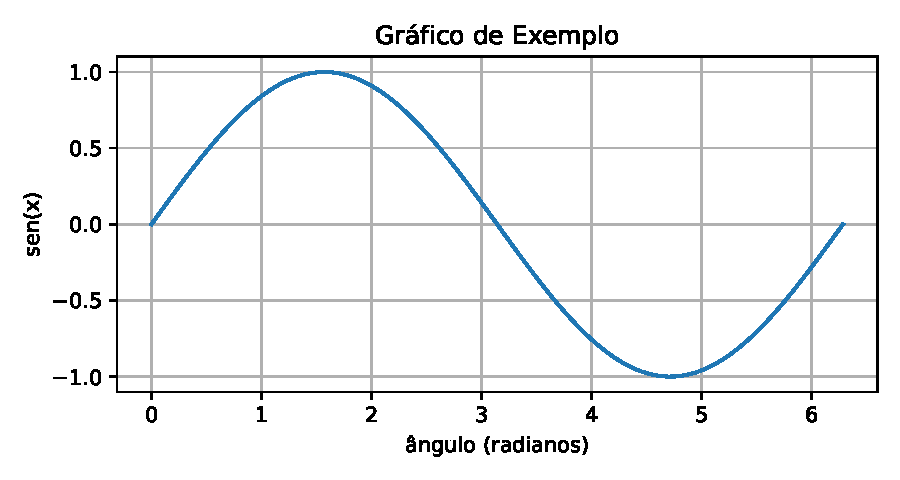
\includegraphics[scale=1.0]{figs/seno}
\end{center}

Mais informações sobre os recursos de \inlcode{Matplotlib} podem ser encontradas na documentação oficial da biblioteca,
disponível em: \colorurl{https://matplotlib.org/stable/contents.html}.

Assim como a na biblioteca \inlcode{Matplotlib}, os exemplos apresentados acima têm como objetivo apenas introduzir a
\inlcode{NumPy}.
Ela oferece uma ampla gama de funcionalidades não abordadas, incluindo muitas outras operações vetoriais, manipulação
de arrays multidimensionais, transformações estruturais, mapeamento e interpolação de valores, entre muitos outros
recursos voltados à computação numérica.
Recomenda-se que o leitor explore essas funcionalidades conforme sua necessidade.
A documentação oficial da biblioteca está disponível em: \colorurl{https://numpy.org/doc}.


Além disso, recomenda-se ao leitor explorar a biblioteca \inlcode{SciPy}, que complementa e expande as funcionalidades
do \inlcode{NumPy} ao disponibilizar ferramentas especializadas para áreas como álgebra linear, equações diferenciais,
integração numérica, otimização, interpolação, transformadas e processamento de sinais.
A documentação oficial da biblioteca está disponível em: \colorurl{https://docs.scipy.org/doc/scipy/}.


